\documentclass[]{article}
\usepackage{amsmath, amsfonts, amssymb, amsthm}
\usepackage{cancel}
\usepackage{siunitx}
\usepackage[american]{circuitikz}
\usepackage{bm}
\usepackage{graphicx}
\usepackage{pgfplots}
\usepackage{pdfpages}

\renewcommand{\thesection}{\arabic{section}}
\renewcommand{\thesubsection}{\thesection.\alph{subsection}}
\renewcommand{\thesubsubsection}{\thesubsection.\roman{subsubsection}}

\newtheorem{genthm}{Theorem}

\newcommand{\unit}[1]{\bm{\hat{#1}}}
\newcommand{\iprod}[2]{\left\langle #1, #2 \right\rangle}
\newcommand{\tpose}[1]{#1^{\! \top} \!}

\title{EECS 16B HW00}
\author{Bryan Ngo}
\date{2020-01-25}

\begin{document}

\maketitle

\section{Tell Us Something You are Proud of this Semester}

I am proud to have moved on to 2nd semester.

\section{What are You Looking Forward to Over Winter Break?}

Meeting old friends and family.

\section{Where is the Sound Coming From?}

\subsection{}

We can determine that the time delay \(\Delta t_1 = \SI{9}{\milli\second}\) and \(\Delta t_2 = \SI{11}{\milli\second}\).
Then,
\begin{align}
	d_1 &= v_s \Delta t_1 = (\SI{300}{\meter\per\second})(\SI{9}{\milli\second}) = \SI{2.7}{\meter} \\
	d_2 &= v_s \Delta t_2 = (\SI{300}{\meter\per\second})(\SI{11}{\milli\second}) = \SI{3.3}{\meter}
\end{align}

\subsection{}

Using trigonometry,
\begin{equation}
	\sin(\alpha) = \frac{d}{\|\bm{p}_1\|} = \frac{1}{2}
\end{equation}
making \(\alpha = \sin^{-1}\left(\frac{1}{2}\right) = \frac{\pi}{6} \,  \si{\radian}\).

\subsection{}

Using the trilateration formula
\begin{equation}
	2\begin{bmatrix}
	\tpose{\bm{a}_1 - \bm{a}_2} \\
	\tpose{\bm{a}_1 - \bm{a}_3} \\
	\tpose{\bm{a}_1 - \bm{a}_4}
	\end{bmatrix} \bm{x}
	=
	\begin{bmatrix}
	\|\bm{a}_1\|^2 - \|\bm{a}_2\|^2 - d_1^2 + d_2^2 \\
	\|\bm{a}_1\|^2 - \|\bm{a}_3\|^2 - d_1^2 + d_3^2 \\
	\|\bm{a}_1\|^2 - \|\bm{a}_4\|^2 - d_1^2 + d_4^2
	\end{bmatrix}
\end{equation}
We then plug in our values,
\begin{align}
	2\begin{bmatrix}
	\tpose{\left(\begin{bmatrix}
		0 \\
		4
		\end{bmatrix}
		-
		\begin{bmatrix}
		0 \\
		2
		\end{bmatrix}\right)} \\
	\tpose{\left(\begin{bmatrix}
		0 \\
		4
		\end{bmatrix}
		-
		\begin{bmatrix}
		0 \\
		1
		\end{bmatrix}\right)} \\
	\tpose{\left(\begin{bmatrix}
		0 \\
		4
		\end{bmatrix}
		-
		\begin{bmatrix}
		0 \\
		0
		\end{bmatrix}\right)}
	\end{bmatrix} \bm{x}
	&=
	\begin{bmatrix}
	16 - 4 - 1 + 5 \\
	16 - 1 - 1 + 10 \\
	16 - 0 - 1 + 17
	\end{bmatrix} \\
	2\begin{bmatrix}
	\tpose{\begin{bmatrix}
		0 \\
		2
		\end{bmatrix}} \\
	\tpose{\begin{bmatrix}
		0 \\
		3
		\end{bmatrix}} \\
	\tpose{\begin{bmatrix}
		0 \\
		4
		\end{bmatrix}}
	\end{bmatrix} \bm{x}
	&=
	\begin{bmatrix}
	16 \\
	24 \\
	32
	\end{bmatrix} \\
	\begin{bmatrix}
	0 & 2 \\
	0 & 3 \\
	0 & 4
	\end{bmatrix} \bm{x}
	=
	\begin{bmatrix}
	8 \\
	12 \\
	16
	\end{bmatrix}
\end{align}
Using least squares,
\begin{align}
	\tpose{\bm{A}} \bm{A} = 
	\begin{bmatrix}
	0 & 0 & 0 \\
	2 & 3 & 4
	\end{bmatrix}
	\begin{bmatrix}
	0 & 2 \\
	0 & 3 \\
	0 & 4
	\end{bmatrix}
	=
	\begin{bmatrix}
	0 & 0 \\
	0 & 29
	\end{bmatrix}
\end{align}
Since the matrix is non-invertible (\(\det(\tpose{\bm{A}} \bm{A}) = 0\)), we cannot use least squares to determine the location of the transmitter.
An alternative solution would be to place the microphones in non-collinear locations, so as to make the matrix linearly dependent and thus invertible.

\section{Building a Classifier}

\subsection{}

We construct the least squares problem
\begin{equation}
	\begin{bmatrix}
	-2 & 1 & 1 \\
	-1 & 1 & 1 \\
	1 & 1 & 1 \\
	2 & 1 & 1
	\end{bmatrix}
	\begin{bmatrix}
	\alpha \\
	\beta \\
	\gamma
	\end{bmatrix}
	=
	\begin{bmatrix}
	-1 \\
	1 \\
	1 \\
	-1
	\end{bmatrix}
\end{equation}
Using the least squares formula,
\begin{align}
	\tpose{\bm{A}} \bm{A} =
	\begin{bmatrix}
	-2 & -1 & 1 & 2 \\
	1 & 1 & 1 & 1 \\
	1 & 1 & 1 & 1
	\end{bmatrix}
	\begin{bmatrix}
	-2 & 1 & 1 \\
	-1 & 1 & 1 \\
	1 & 1 & 1 \\
	2 & 1 & 1
	\end{bmatrix}
	=
	\begin{bmatrix}
	10 & 0 & 0 \\
	0 & 4 & 4 \\
	0 & 4 & 4
	\end{bmatrix}
\end{align}
The problem is unsolvable, since columns 2 and 3 are linearly dependent.
This makes \(\tpose{\bm{A}} \bm{A}\) non-invertible.

\subsection{}

\begin{center}
\begin{tikzpicture}
	\begin{axis}[
		xlabel = {\(x_i\)},
		ylabel = {\(y_i\)},
		xmin = -3, xmax = 3,
		ymin = 0, ymax = 3,
		xtick = {-5,...,3},	ytick = {0,..., 3},
		axis lines = middle,
		xmajorgrids = true, ymajorgrids = true,
		grid style = dashed
	]
		\addplot[only marks, color=blue] table {
			-2 1
			-1 1
			1 1
			2 1
		};
		\node[above] at (axis cs: -2, 1) {\(-1\)};
		\node[above] at (axis cs: -1, 1) {\(1\)};
		\node[above] at (axis cs: 1, 1) {\(1\)};
		\node[above] at (axis cs: 2, 1) {\(-1\)};
	\end{axis}
\end{tikzpicture}
\end{center}
From the diagram, it is clear that it is impossible to draw a line that uniquely classifies the points by label.

\subsection{}

We set up the least squares problem
\begin{equation}
	\begin{bmatrix}
	-2 & 4 \\
	-1 & 1 \\
	1 & 1 \\
	2 & 4
	\end{bmatrix}
	\begin{bmatrix}
	\alpha \\
	\beta
	\end{bmatrix}
	=
	\begin{bmatrix}
	-1 \\
	1 \\
	1 \\
	-1
	\end{bmatrix}
\end{equation}
Using least squares,
\begin{align}
	\tpose{\bm{A}} \bm{A} &=
	\begin{bmatrix}
	-2 & -1 & 1 & 2 \\
	4 & 1 & 1 & 4
	\end{bmatrix}
	\begin{bmatrix}
	-2 & 4 \\
	-1 & 1 \\
	1 & 1 \\
	2 & 4
	\end{bmatrix}
	=
	\begin{bmatrix}
	10 & 0 \\
	0 & 34
	\end{bmatrix}
	\overset{-1}{\Rightarrow}
	\begin{bmatrix}
	\frac{1}{10} & 0 \\
	0 & \frac{1}{34}
	\end{bmatrix} \\
	\tpose{\bm{A}} \bm{b} &=
	\begin{bmatrix}
	-2 & -1 & 1 & 2 \\
	4 & 1 & 1 & 4
	\end{bmatrix}
	\begin{bmatrix}
	-1 \\
	1 \\
	1 \\
	-1
	\end{bmatrix}
	=
	\begin{bmatrix}
	0 \\
	-6
	\end{bmatrix} \\
	\unit{x} &= (\tpose{\bm{A}} \bm{A})^{-1} \tpose{\bm{A}} \bm{b} =
	\begin{bmatrix}
	\frac{1}{10} & 0 \\
	0 & \frac{1}{34}
	\end{bmatrix}
	\begin{bmatrix}
	0 \\
	-6
	\end{bmatrix}
	=
	\begin{bmatrix}
	0 \\
	-\frac{6}{34}
	\end{bmatrix} \\
	\ell &\approx -\frac{3}{17} x^2
\end{align}

\subsection{}

\begin{center}
\begin{tikzpicture}
	\begin{axis}[
		xlabel = {\(x_i\)},
		ylabel = {\(x_i^2\)},
		xmin = -3, xmax = 3,
		ymin = 0, ymax = 5,
		xtick = {-3,...,3},	ytick = {0,..., 5},
		axis lines = middle,
		xmajorgrids = true, ymajorgrids = true,
		grid style = dashed
	]
		\addplot[only marks, color=blue] table {
			-2 4
			-1 1
			1 1
			2 4
		};
		\node[above] at (axis cs: -2, 4) {\(-1\)};
		\node[above] at (axis cs: -1, 1) {\(1\)};
		\node[above] at (axis cs: 1, 1) {\(1\)};
		\node[above] at (axis cs: 2, 4) {\(-1\)};
		\addplot[
			domain = -5:5,
			samples = 100,
			color = red
		]
		{2.5};
	\end{axis}
\end{tikzpicture}
\end{center}
It is possible to classify the labels using a quadratic regression.

\subsection{}

Using the model \(\ell = \alpha x + \beta x^2 + \gamma\) would create a more accurate classifier.
This is due to the extra degree of freedom gained by the \(\gamma\) term.

\section{Putting on the Pressure: Build Your Own InstantPot}

\subsection{}

\begin{equation}
	R_p = \frac{\rho L}{A} = \frac{\SI{0.1}{\ohm\meter} \cdot  \SI{0.01}{\meter}}{\SI{0.001}{\meter} \cdot \SI{100d-6}{\meter}} = \SI{d4}{\ohm}
\end{equation}

\subsection{}

\begin{equation}
	R_p(p_c) = \frac{\rho L(p_c)}{W t} = \frac{\rho}{W t} (L_0 + \beta p_c)
\end{equation}

\subsection{Pressure Sensor Circuit}

\begin{center}
\begin{circuitikz} \draw
	(0, 0) node[op amp] (opamp) {}
	(opamp.-) to[short] (-1.19, 1.5)
	(-1.19, 1.5) to[R=\(R_p\)] (1.19, 1.5)
	(1.19, 1.5) to[short] (opamp.out)
	(opamp.out) to[short] (2, 0)
	(2, -2) node[ground]{}
	(2, 0) to[open, v^=\(V_p\), o-o] (2, -2)
	(opamp.+) node[ground]{}
	(-3, 0) to[V=\(V_0\)] (-3, -1) node[ground] {}
	(-3, 0) to[short] (-3, 0.5) to[R=\(R_z\)] (opamp.-)
;\end{circuitikz}
\end{center}
Recognizing that this is an inverting op-amp, we can use the formula
\begin{equation}
	V_p = -V_0 \frac{R_p}{R_z}
\end{equation}
and solve for \(R_z\).
Plugging in our values of \(R_p\),
\begin{equation}
	V_p = -V_0 \frac{R_0 \frac{p_c}{p_{ref}}}{R_z} = -V_0 \frac{p_c}{p_{ref}} \frac{R_0}{R_z}
\end{equation}
In order to satisfy our desired voltage of \(V_p = -V_0 \frac{p_c}{p_{ref}}\), \(\frac{R_0}{R_z} = 1\).
Thus, \(R_z = R_0 = \SI{1}{\kilo\ohm}\).

\subsection{Resistive Heating Element}

\begin{equation}
	P = \frac{V_{heat}^2}{R_{heat}} \Rightarrow \SI{1000}{\watt} = \frac{\SI{100}{\volt}^2}{R_{heat}}
\end{equation}	
yielding \(R_{heat} = \SI{10}{\ohm}\).

\subsection{Pressure Regulation}

\begin{center}
	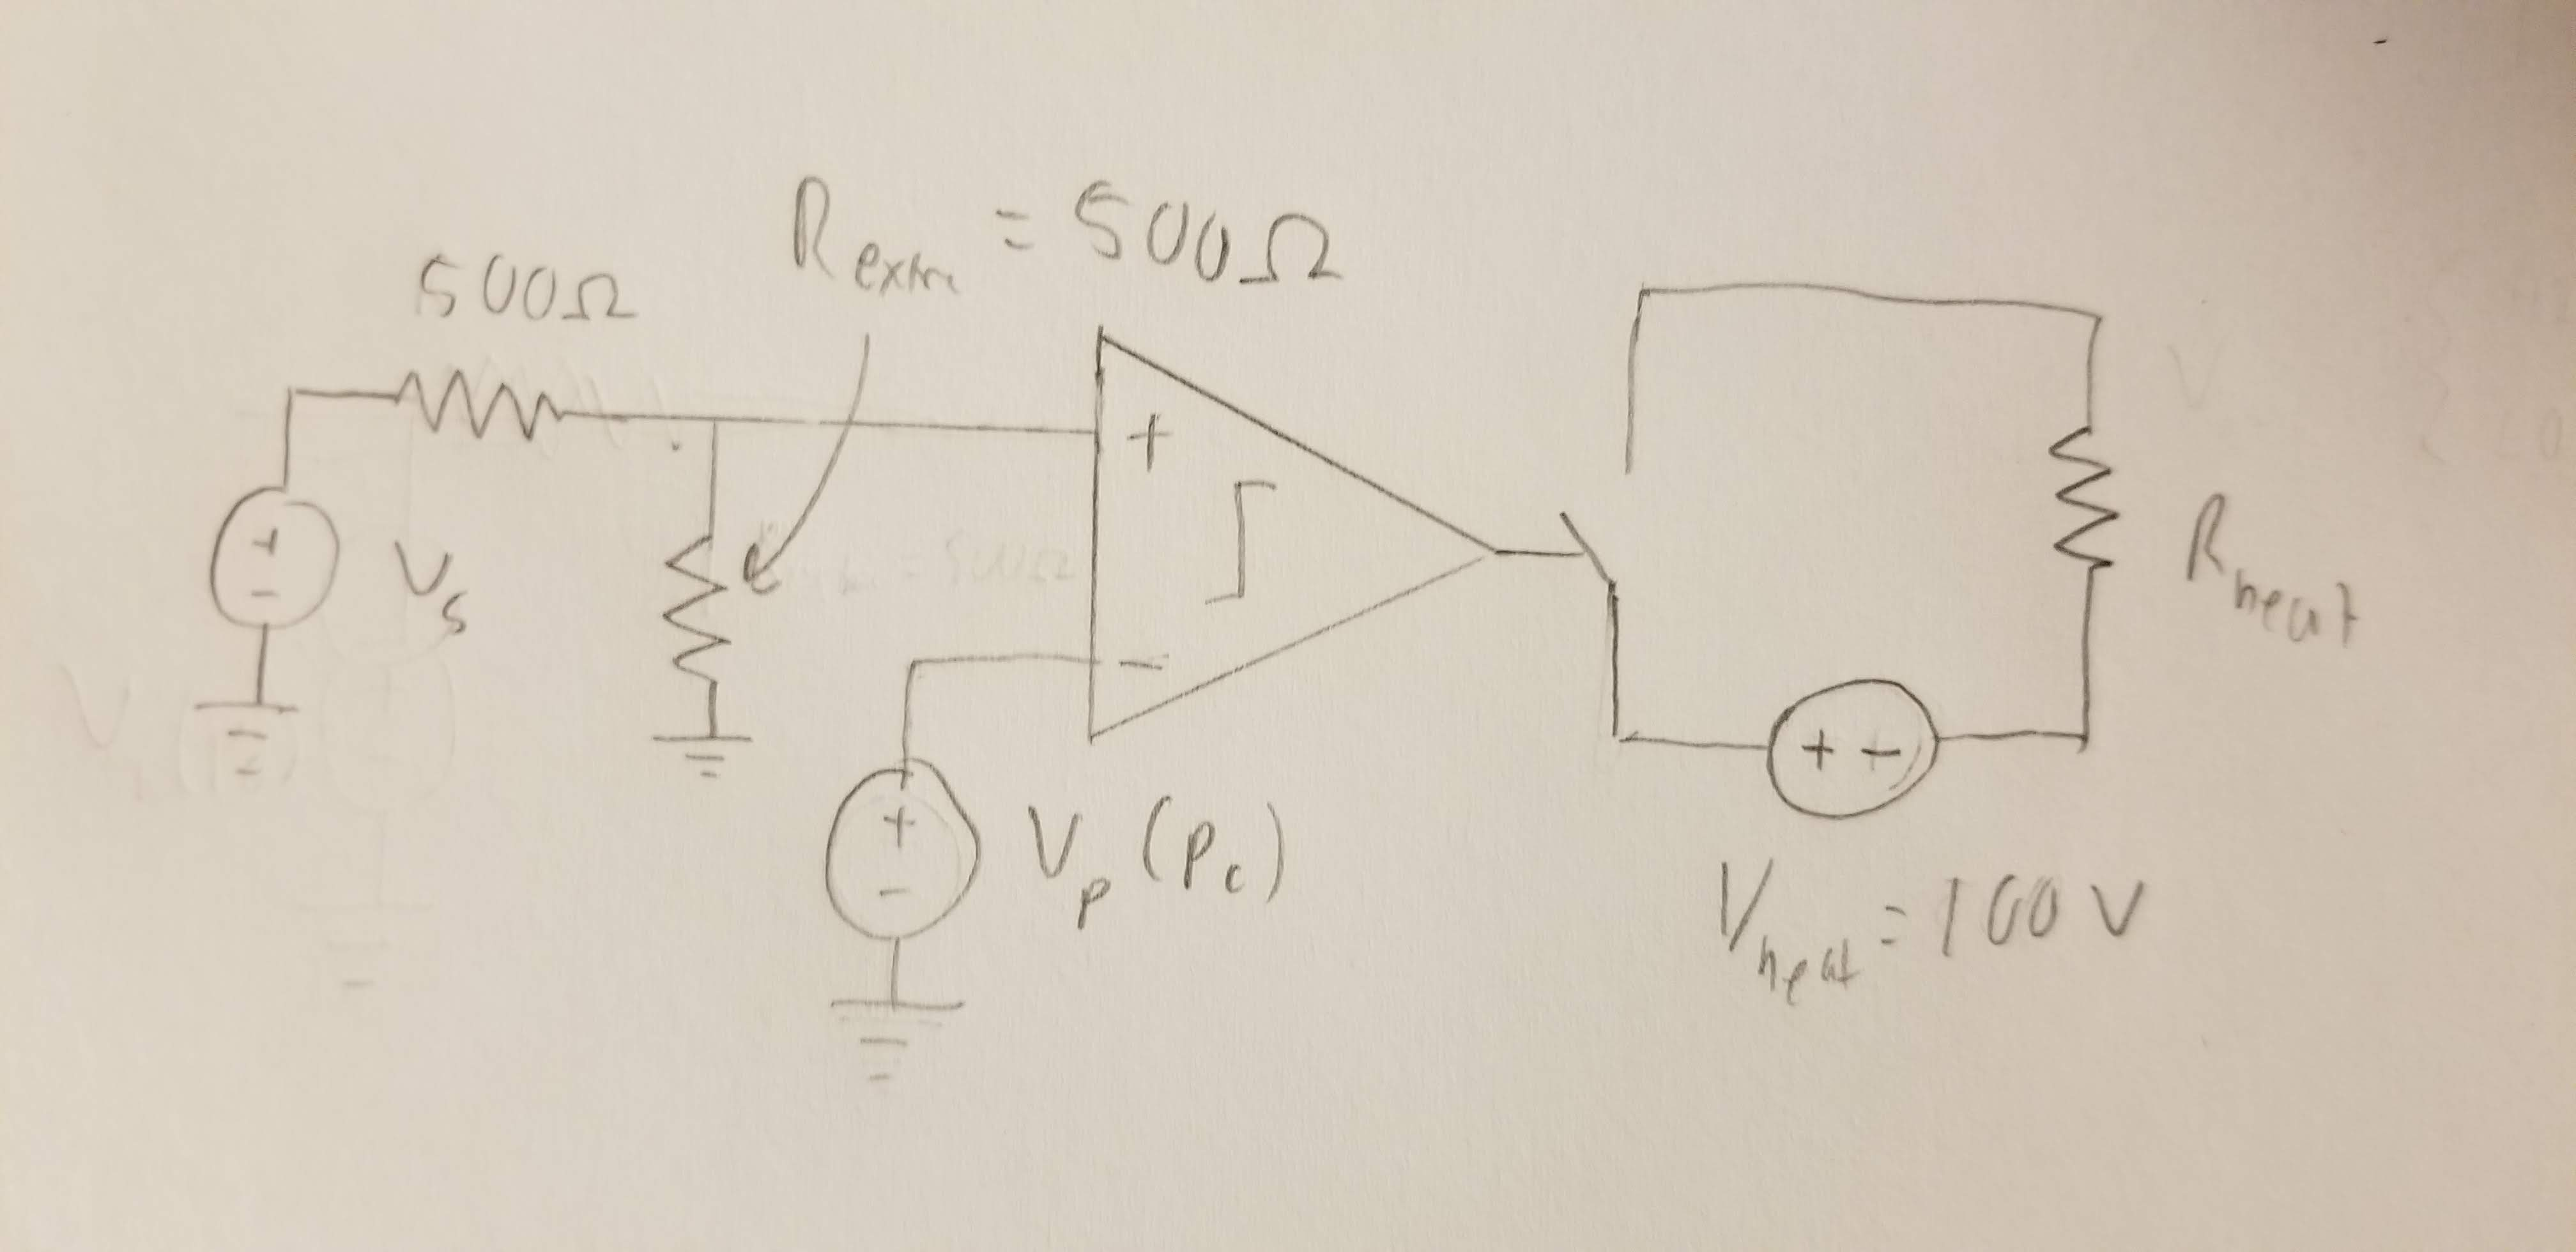
\includegraphics[width=0.7\linewidth]{20200125_170202}
\end{center}

\section{Finding Faults with PG\&E}

\subsection{}

\begin{center}
\begin{tikzpicture}
	\begin{axis}[
		xlabel = {\(k\)},
		ylabel = {\(\operatorname{corr}_{\bm{r}}(\bm{t})[k]\)},
		xmin = -5, xmax = 5,
		ymin = -5, ymax = 10,
		xtick = {-5,...,5},	ytick = {-5,..., 10},
		axis lines = middle,
		ymajorgrids = true,
		grid style = dashed
	]
		\addplot[
			ycomb,
			color=blue,
			mark=*
		]
		coordinates {
			(-3, 0)
			(-2, 0)
			(-1, 0)
			(0, -3)
			(1, 8)
			(2, -4)
			(3, 0)
		};
	\end{axis}
\end{tikzpicture}
\end{center}
The index of the maximum correlation is \(k = 1\).

\subsection{}

Using OMP, we first find the largest magnitude of the inner product \(\iprod{\bm{r}}{\bm{u}_i}\), which is \(i = 1\).
Finding our preliminary "weight",
\begin{align}
	\tpose{\bm{A}} \bm{A} &= \|\bm{u}_1\|^2 = 3 \\
	\tpose{\bm{A}} \bm{r} &= \iprod{\bm{u}_1}{\bm{r}} = 5 \\
	\unit{x} &= (\tpose{\bm{A}} \bm{A})^{-1} \tpose{\bm{A}} \bm{r} = \frac{5}{3}
\end{align}
Finding our new error vector,
\begin{equation}
	\bm{r}' = \bm{r} - \bm{A}\unit{x} =
	\begin{bmatrix}
	1 \\
	2 \\
	1 \\
	2 \\
	1
	\end{bmatrix}
	-
	\frac{5}{3}\begin{bmatrix}
	0 \\
	1 \\
	1 \\
	1 \\
	0
	\end{bmatrix}
	=
	\begin{bmatrix}
	1 \\
	\frac{1}{3} \\
	-\frac{2}{3} \\
	\frac{1}{3} \\
	1
	\end{bmatrix}
\end{equation}
Our new maximum inner product is
\[\begin{array}{c|c}
	i & \iprod{\bm{r}'}{\bm{u}_i} \\
	\hline
	1 & 0 \\
	2 & 0 \\
	3 & \frac{2}{3} \\
	4 & \frac{4}{3}
\end{array}\]
Then, we use least squares to find the weights,
\begin{align}
	\tpose{\bm{A}} \bm{A} &=
	\begin{bmatrix}
	0 & 1 & 1 & 1 & 0 \\
	0 & 0 & -1 & -1 & 1
	\end{bmatrix}
	\begin{bmatrix}
	0 & 0 \\
	1 & 0 \\
	1 & -1 \\
	1 & -1 \\
	0 & 1
	\end{bmatrix} =
	\begin{bmatrix}
	3 & -2 \\
	-2 & 3
	\end{bmatrix}
	\overset{-1}{\Rightarrow}
	\frac{1}{5}\begin{bmatrix}
	3 & 2 \\
	2 & 3
	\end{bmatrix} \\
	\tpose{\bm{A}} \bm{r} &= 
	\begin{bmatrix}
	0 & 1 & 1 & 1 & 0 \\
	0 & 0 & -1 & -1 & 1
	\end{bmatrix}
	\begin{bmatrix}
	1 \\
	2 \\
	1 \\
	2 \\
	1
	\end{bmatrix}
	=
	\begin{bmatrix}
	5 \\
	-2
	\end{bmatrix} \\
	\unit{x} &= (\tpose{\bm{A}} \bm{A})^{-1} \tpose{\bm{A}} \bm{r} =
	\frac{1}{5}\begin{bmatrix}
	3 & 2 \\
	2 & 3
	\end{bmatrix}
	\begin{bmatrix}
	5 \\
	-2
	\end{bmatrix}
	=
	\frac{1}{5}\begin{bmatrix}
	11 \\
	4
	\end{bmatrix}
\end{align}
So our signal \(\bm{r} = \frac{11}{5}\bm{u}_1 + \frac{4}{5}\bm{u}_4\).

\section{Fun with Circuits}

\subsection{Equivalent Resistance}

If we apply a test voltage \(V_{test}\) at \(V_1\),
\begin{center}
\begin{circuitikz} \draw
	(0, 2) to[open, v=\(V_{test}\)] (0, 0)
	(0, 2) node[ocirc]{\(A\)} to[R=\SI{1}{\kilo\ohm}, i=\!] (2, 2) to[R=\SI{4}{\kilo\ohm}, i=\!] (4, 2) to[cvsource, v=\(3V_2\)] (4, 0) to[short] (0, 0) node[ocirc]{\(B\)}
	(2, 2) to[open, v=\(V_2\), *-*] (2, 0)
;\end{circuitikz}
\end{center}
The NVA equations are
\begin{align}
	I_{R_2} - I_{R_1} &= 0 \\
	 \frac{V_2 - 3V_2}{\SI{4}{\kilo\ohm}} - \frac{V_{test} - V_2}{\SI{1}{\kilo\ohm}}&= 0 \\
	 - \frac{V_2}{\SI{2}{\kilo\ohm}} - \frac{V_{test}}{\SI{1}{\kilo\ohm}} + \frac{V_2}{\SI{1}{\kilo\ohm}} &= 0 \\
	V_2 &= 2V_{test} \\
	I_{R_1} &= \frac{V_{test} - 2V_{test}}{\SI{1}{\kilo\ohm}} = -\frac{V_{test}}{\SI{1}{\kilo\ohm}} \\
	R_{eq} &= \frac{V_{test}}{I_{R_1}} = \SI{-1}{\kilo\ohm}
\end{align}

\subsection{Amplifier Design}

\begin{center}
\begin{circuitikz} \draw
	(0, 0) node[op amp, yscale=-1] (opamp) {}
	(opamp.-) to[short] (-1.19, -4) to[short] (1.19, -4)
	(opamp.out) to[R=\SI{1}{\kilo\ohm}] (1.19, -2) to[R=\SI{1}{\kilo\ohm}] (1.19, -4) to[R=\SI{1}{\kilo\ohm}] (1.19, -6) node[ground]{}
	(opamp.out) to[short] (2, 0)
	(2, -2) node[ground]{}
	(2, 0) to[open, v^=\(3V_0\), o-o] (2, -2)
	(-3, 0) to[sV=\(V_0\)] (-3, -1) node[ground] {}
	(-3, 0) to[short] (-3, 0.49) to[short] (opamp.+)
;\end{circuitikz}
\end{center}
As a non-inverting amplifier,
\begin{align}
	V_{out} &= V_{in}\left(1 + \frac{R_t}{R_b}\right) \\
	&= V_{in}\left(1 + \frac{\SI{2}{\kilo\ohm}}{\SI{1}{\kilo\ohm}}\right) = 3V_{in}
\end{align}

\section{Projections and Eigenvectors}

\subsection{}

The matrix \(\bm{M} = \bm{x} \tpose{\bm{y}} \in \mathbb{R}^{n \times n}\).

\subsection{}

\begin{align}
	\bm{M} &=
	\begin{bmatrix}
	1 \\
	2
	\end{bmatrix}
	\begin{bmatrix}
	4 & 5
	\end{bmatrix}
	=
	\begin{bmatrix}
	4 & 5 \\
	8 & 10
	\end{bmatrix} \\
	\Rightarrow \begin{vmatrix}
	4 - \lambda & 5 \\
	8 & 10 - \lambda
	\end{vmatrix} &= 0 \\
	(4 - \lambda) (10 - \lambda) - 40 &= 0 \\
	40 - 4\lambda - 10\lambda + \lambda^2 - 40 &= 0 \\
	\lambda^2 - 14\lambda &= 0 \\
	\lambda &= 0, 14
\end{align}
Finding the eigenvectors,
\begin{align}
	&\left[\begin{array}{@{}cc|c@{}}
	4 & 5 & 0 \\
	8 & 10 & 0
	\end{array}\right] \\
	\overset{r_2 - 2r_1 \to r_2}{\Longrightarrow}
	&\left[\begin{array}{@{}cc|c@{}}
	4 & 5 & 0 \\
	0 & 0 & 0
	\end{array}\right] \\
	\bm{e}_1 &= \operatorname{span}\left\{\begin{bmatrix}
	-\frac{5}{4} \\
	1
	\end{bmatrix}\right\} \\
	&\left[\begin{array}{@{}cc|c@{}}
	-10 & 5 & 0 \\
	8 & -4 & 0
	\end{array}\right] \\
	\overset{r_1/-5 \to r_1, r_2/4 \to r_2}{\Longrightarrow}
	&\left[\begin{array}{@{}cc|c@{}}
	2 & -1 & 0 \\
	2 & -1 & 0
	\end{array}\right] \\
	\overset{r_2 - r_1 \to r_2}{\Longrightarrow}
	&\left[\begin{array}{@{}cc|c@{}}
	2 & -1 & 0 \\
	0 & 0 & 0
	\end{array}\right] \\
	\bm{e}_2 &= \operatorname{span}\left\{\begin{bmatrix}
	\frac{1}{2} \\
	1
	\end{bmatrix}\right\}
\end{align}

\subsection{}

\begin{align}
	\operatorname{proj}_{\bm{M}}(\bm{x}) &= \bm{M}(\tpose{\bm{M}} \bm{M})^{-1} \tpose{\bm{M}} \bm{x} \\
	&= \bm{M}(\tpose{(\bm{x} \tpose{\bm{y}})} \bm{x} \tpose{\bm{y}})^{-1} \tpose{(\bm{x} \tpose{\bm{y}})} \bm{x} \\
	&= \bm{M}(\bm{y} \tpose{\bm{x}} \bm{x} \tpose{\bm{y}})^{-1} \bm{y} \tpose{\bm{x}} \bm{x} \\
	&= \bm{M}(\cancel{\|\bm{x}\|^2} \bm{y} \tpose{\bm{y}})^{-1} \bm{y} \cancel{\|\bm{x}\|^2} \\
	&= \bm{x}\tpose{\bm{y}}(\bm{y} \tpose{\bm{y}})^{-1}\bm{y} \\
	&= \bm{x}
\end{align}

\subsection{}

\begin{genthm}
	Suppose \(\bm{x}, \bm{y} \in \mathbb{R}^n\) and \(\bm{M} = \bm{x} \tpose{\bm{y}}\).
	Then, for some \(\bm{z} \in \mathbb{R}^n\) such that \(\iprod{\bm{z}}{\bm{y}} = 0\), \(\bm{z} \in \operatorname{null}(\bm{M})\). 
\end{genthm}

\begin{proof}
\begin{align}
	\iprod{\bm{z}}{\bm{y}} = \iprod{\bm{y}}{\bm{z}} &= 0 && \text{commutativity of inner product} \\
	\tpose{\bm{y}} \bm{z} &= 0 && \text{definition of inner product} \\
	\bm{x} \tpose{\bm{y}} \bm{z} &= 0 && \text{multiply by } \bm{x} \text{ on both sides} \\
	\bm{M} \bm{z} &= 0 && \text{definition of } \bm{M} \\
	\bm{z} &\in \operatorname{null}(\bm{M}) && \text{definition of nullspace}
\end{align}
\end{proof}

\subsection{}

\begin{align}
	\bm{M} &=
	\begin{bmatrix}
	y_1 \bm{x} & y_2 \bm{x} & \cdots & y_n \bm{x}
	\end{bmatrix} \\
	\bm{Mx} &=
	\begin{bmatrix}
	y_1 \bm{x} & y_2 \bm{x} & \cdots & y_n \bm{x}
	\end{bmatrix}
	\begin{bmatrix}
	x_1 \\
	x_2 \\
	\cdots \\
	x_n
	\end{bmatrix} \\
	&= x_1 y_1 \bm{x} + x_2 y_2 \bm{x} + \cdots + x_n y_n \bm{x} \\
	&= \sum_{i = 1}^n x_i y_i \bm{x} \\
	&= \iprod{\bm{x}}{\bm{y}} \bm{x}
\end{align}
We find that \(\bm{M}\) as eigenvector \(\bm{x}\) with eigenvalue \(\iprod{\bm{x}}{\bm{y}}\).

\section{Electronic Level}

\begin{center}
\begin{circuitikz} \draw
	(0, 2) to[V_=\(V_s\)] (0, 0) to[short] (8, 0) to[V_=\(-V_s\), invert] (8, 2)
	(0, 2) to[nos] (2, 2) to[nos] (4, 2) to[nos] (6, 2) to[nos] (8, 2)
	(2, 2) to[C=\(C_a\), v=\(V_a\)] (2, 0)
	(4, 2) to[C=\(C_1\), v=\(V_{out}\)] (4, 0)
	(6, 2) to[C=\(C_b\), v=\(V_b\)] (6, 0)
;\end{circuitikz}
\end{center}

\subsection{}

During phase 1,
\begin{center}
\begin{circuitikz} \draw
	(0, 2) to[V_=\(V_s\)] (0, 0) to[short] (8, 0) to[V_=\(-V_s\), invert] (8, 2)
	(0, 2) to[short] (2, 2) to[nos] (4, 2) to[nos] (6, 2) to[short] (8, 2)
	(2, 2) to[C=\(C_a\), v=\(V_a\)] (2, 0)
	(4, 2) to[C=\(C_1\), v=\(V_{out}\)] (4, 0)
	(6, 2) to[C=\(C_b\), v=\(V_b\)] (6, 0)
;\end{circuitikz}
\end{center}
which leaves the capacitors with charge
\begin{align}
	Q_a &= C_a V_s \\
	Q_b &= -C_b V_s \\
	Q_{tot}(0) = Q_{tot}(1) &= V_s(C_a - C_b)
\end{align}
Plugging in our values of \(C_a\) and \(C_b\),
\begin{align}
	V_s (C_a - C_b) &= V_s \left(C_0 \left(100 + \frac{\alpha}{\alpha_{ref}}\right) - C_0 \left(100 - \frac{\alpha}{\alpha_{ref}}\right)\right) \\
	&= V_s\left(\cancel{100C_0} + C_0\frac{\alpha}{\alpha_{ref}} - \cancel{100C_0} + C_0\frac{\alpha}{\alpha_{ref}}\right) \\
	&= 2C_0V_s \frac{\alpha}{\alpha_{ref}}
\end{align}

\subsection{}

\begin{align}
	V_{out}(1) &= \frac{Q_{tot}(1)}{\underbrace{C_a + C_b + C_1}_{\text{in parallel}}} \\
	&= \frac{Q_{tot}(1)}{C_0 \left(100 + \frac{\alpha}{\alpha_{ref}}\right) + C_0 \left(100 - \frac{\alpha}{\alpha_{ref}}\right)} \\
	&= \frac{Q_{tot}(1)}{200C_0 + C_1}
\end{align}

\subsection{}

We can construct the equation for the total charge on the capacitor as
\begin{equation}
	Q_{tot}(k) = Q_{tot}(k - 1) + V_s(C_a - C_b)
\end{equation}
Then, plugging into the equation in \textbf{7.b}, we get
\begin{align}
	V_{tot}(k) &= \frac{Q_{tot}(k - 1) + 2 C_0 V_s \frac{\alpha}{\alpha_{ref}}}{200C_0 + C_1} \\
	&= \frac{C_1 V_{out}(k - 1) + 2 C_0 V_s \frac{\alpha}{\alpha_{ref}}}{200C_0 + C_1}
\end{align}

\subsection{}

By induction,
\begin{align}
	V_{out}(1) &= \gamma V_{out}(0) + \beta = \beta \\
	V_{out}(2) &= \gamma \beta + \beta \\
	V_{out}(3) &= \gamma (\gamma \beta + \beta) + \beta = \gamma^2 \beta + \gamma \beta + \beta \\
	&\vdots \\
	\lim_{k \to \infty} V_{out}(k) &= \sum_{i = 0}^{\infty} \beta \gamma^i = \frac{\beta}{1 - \gamma}
\end{align}

\section{Homework Process and Study Group}

\subsection{}

I used notes from EECS 16A to assist me with the homework.

\subsection{}

I did this homework by myself.

\subsection{}

I spent 3 hours doing the homework, then went to eat dinner.
Afterwards, I finished the homework in 2 hours.

\subsection{}

It took me 5 hours to do this homework.

\newpage

%\includepdf[pages=-]{prob*.pdf}

\end{document}
